\documentclass{article}
\usepackage{amsmath,amssymb,graphicx,algpseudocode,algorithm,amsthm}
\usepackage[margin=1in]{geometry}
\usepackage{mathrsfs}
\let\mathcrl\mathscr
\usepackage[mathscr]{euscript}
\usepackage{marginnote}
\usepackage{hyperref}
\usepackage{qtree}
\usepackage{graphicx}
\usepackage{tikz}
\geometry{reversemarginpar}


\author{Benji Altman}

\def\latex{\LaTeX\ }

\def\useLim{\limits}
\newcommand{\question}[1]{\marginnote{#1}}
\let\union\cup
\let\inter\cap
\let\emptyset\varnothing
\let\bigunion\bigcup
\let\biginter\bigcap
\let\composed\circ
\let\cross\times
\def\And{\textit{ and }}
\def\Or{\textit{ or }}
\def\sbSeperator{\,\middle|\,}
\def\Return{\State\textbf{return}\par}
\def\ZNonNegative{{\mathbb Z_{\ge 0}}}
\newcommand{\setcomp}[1]{{#1}^{\mathsf{c}}}
\newcommand{\prodfrom}[3]{\prod\useLim_{#1}^{#2}\LB {#3} \RB}
\newcommand{\sumfrom}[3]{\sum\useLim_{#1}^{#2} \LB {#3} \RB}
\newcommand{\unionfrom}[3]{\bigunion\useLim_{#1}^{#2} \LB {#3} \RB}
\newcommand{\interfrom}[3]{\biginter\useLim_{#1}^{#2} \LB {#3} \RB}
\newcommand{\interacross}[2]{\interfrom{#1}{}{#2}}
\newcommand{\unionacross}[2]{\unionfrom{#1}{}{#2}}
\newcommand{\sumacross}[2]{\sumfrom{#1}{}{#2}}
\newcommand{\prodacross}[2]{\prodfrom{#1}{}{#2}}
\newcommand{\Lim}[3]{\lim\useLim_{{#1} \to {#2}}\LB {#3} \RB}
\newcommand{\set}[1]{\left\{ {#1} \right\}}
\newcommand{\setbuilder}[2]{\left\{{#1} \sbSeperator {#2}\right\}}
\newcommand{\derivative}[2]{\frac{d}{d{#2}}\LB {#1} \RB}
\newcommand{\Exists}[2]{\exists_{#1}\LB {#2} \RB}
\newcommand{\All}[2]{\forall_{#1}\LB {#2} \RB}
\newcommand{\abs}[1]{\left|{#1}\right|}
\newcommand{\card}[1]{\left| {#1} \right|}
\newcommand{\range}[1]{\textit{\textbf{Rng}}\left( {#1} \right)}
\newcommand{\domain}[1]{\textit{\textbf{Dom}}\left( {#1} \right)}
\newcommand{\pset}[1]{\mathcal P\left( {#1} \right)}
\newcommand{\pair}[2]{\left( {#1} , {#2} \right)}
\def\closure{\overline}
\newcommand{\limpts}[1]{{#1} '}
\newcommand{\ooint}[2]{\left( {#1} , {#2} \right)}
\newcommand{\ocint}[2]{\left( {#1} , {#2} \right]}
\newcommand{\coint}[2]{\left[ {#1} , {#2} \right)}
\newcommand{\ccint}[2]{\left[ {#1} , {#2} \right]}
\newcommand{\eqclass}[1]{\bar{#1}}
\newcommand{\ceil}[1]{\left\lceil {#1} \right\rceil}
\newcommand{\floor}[1]{\left\lfloor {#1} \right\rfloor}
\newcommand{\inv}[1]{{#1}^{-1}}
\def\true{\text{True}}
\def\false{\text{False}}
\newcommand{\ball}[2]{B_{#1}\left({#2}\right)}
\def\LB{}
\def\RB{}
\newcommand{\cannonicalSet}[1]{\left[ #1 \right]}
\let\lxor\oplus
\newcommand{\norm}[1]{\left|\left|{#1}\right|\right|}

\newtheorem{theorem}{Theorem}[section]
\newtheorem{lemma}[theorem]{Lemma}
\theoremstyle{definition}
\newtheorem{definition}{Definition}[section]

\usepackage[toc,xindy]{glossaries}

\makenoidxglossaries

\newglossaryentry{set}
{
	name={set},
	description={A collection of objects}
}
\newglossaryentry{vertex}
{
	name={vertex},
	description={A point or node in a graph},
	plural={verticies}
}
\newglossaryentry{edge}
{
	name={edge},
	description={A connection or line between verticies in a graph}
}
\newglossaryentry{connected}
{
	name={connected},
	description={A graph where one may start at any point and could follow edges and eventually get to any other point}
}
\newglossaryentry{multigraph}
{
	name={multigraph},
	description={Like a graph, but multiple edges may connect the same vertex pair, and an edge may connect a vertex to itself}
}
\newglossaryentry{complete}
{
	name={complete graph},
	description={A graph with all possible edges included, the notation $K_n$ is used to denote the complete with $n$ verticies}
}
\newglossaryentry{face}
{
	name={face},
	description={An section of the space we are embedding our graph in that is separated from the rest of the space by edges}
}
\newglossaryentry{contraction}
{
	name={contraction},
	description={A graph operation where one removes an edge by fusing two verticies together}
}
\newglossaryentry{subgraph}
{
	name={subgraph},
	description={$A$ is a subgraph of some graph $\mathcal G$ iff you could add verticies and edges to $A$ and somehow get $\mathcal G$}
}
\newglossaryentry{graph}
{
	name={graph},
	description={A set of verticies and edges}
}
\title{Topological Graph Theory}
\begin{document}
\maketitle
\tableofcontents



\section{Introduction}
Topological graph theory is an entire field within topology and as such this paper is by no means meant to cover all of topological graph theory in any depth. This paper instead will first cover a rather shallow overview of the field, followed by a more in depth study of graphs and their genus. The overview will mainly be focused on giving a thorough understanding of what topological graph theory is as well as to briefly cover the history of the field. In giving an overview of the field we will cover some of the basic concepts and definitions needed for the more rigorous part of the paper; as this may be confusing, all definitions will be provided in a glossary at the end. After the overview we will dive into Kuratowski's Theorem, We will go through and attempt to have an intuitive understanding of a Kuratowski's Theorem and it's proof. After proving Kuratowski's Theorem, we will continue onto talking about generalizations of the theorem and map colorings, however their coverage will be rather shallow and lacking proofs.

\section{Overview}
\subsection{Graphs}
Before we talk about topological graph theory with any level of understanding we must first understand what a graph is.

A graph is generally defined as a \gls{set} of \glspl{vertex} combined with a \gls{set} of \glspl{edge} between \glspl{vertex}, however here it may be more useful to think about them visually with a simple representation.

Consider first a \gls{set} of points, this may be thought of as just drawing dots on a sheet of paper. Each of these points will be called a \gls{vertex}. Now we may start drawing lines between \glspl{vertex}. Lines may cross over each other and need not be straight. There is no requirement that all \glspl{vertex} have a line going to it. Each of these lines are called an \gls{edge}. We will simply insist that no \gls{edge} connects two \glspl{vertex} and that we do not have multiple \glspl{edge} between the same pair of \glspl{vertex}.

Once we have drawn this we have a representation of a graph. If we were to move the \glspl{vertex} around on the paper but leave them having the same \glspl{edge} (the same \glspl{vertex} are connected to the point as they were before). we would be left with the same graph. That is to say, it doesn't mater where we put a \gls{vertex} on our sheet, the graph exists independently of the representation we draw.

\subsection{K\"onigsberg, and it's seven bridges}

Consider the following photo-realistic drawing of the city of K\"onigsberg.

\input{Konigsberg.pdf_tex}

Now the question is, if we get to choose where we start, can we go for a stroll and cross every bridge exactly once?

I first came across this question in the 8\textsuperscript{th} grade, and it was presented to us during geometry class. While undoubtedly an interesting problem, it is quite misleading to try and think of this as a geometry problem. Instead we will try and reduce it to a graph problem.

Let us start by thinking of every island as a \gls{vertex} and every bridge as an \gls{edge}. We find the following graph.

\begin{center}
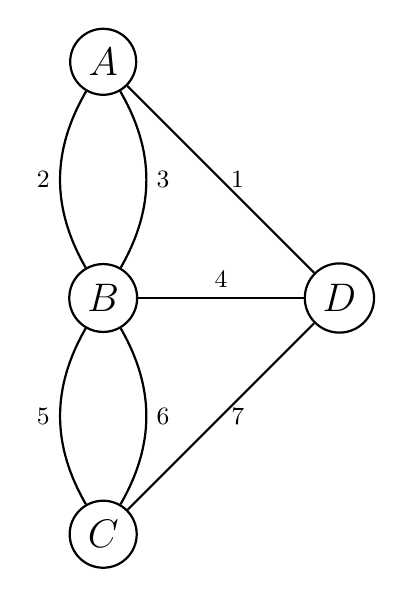
\begin{tikzpicture}[auto, node distance=3cm, every loop/.style={},
                    thick,main node/.style={circle,draw,font=\sffamily\Large\bfseries}]

  \node[main node] (1) {$A$};
  \node[main node] (2) [below of=1] {$B$};
  \node[main node] (3) [below of=2] {$C$};
  \node[main node] (4) [right of=2] {$D$};

  \path[every node/.style={font=\sffamily\small}]
    (1) edge node [right] {$1$} (4)
        edge [bend right] node[left] {$2$} (2)
    (2) edge [bend right] node [right] {$3$} (1)
        edge node {$4$} (4)
        edge [bend right] node[left] {$5$} (3)
    (3) edge [bend right] node [right] {$6$} (2)
    (4) edge node [right] {$7$} (3);
\end{tikzpicture}
\end{center}

It is worth noting two things about the above diagram. First that the labels on the \glspl{vertex} and \glspl{edge} are unrelated to the problem, but have been added simply to make referring to parts of the graph much easier. Second that whatever the above image depicts, does not fit our definition of a graph. %TODO add glossary entry for graph.

Notice that \gls{edge} $2$ and \gls{edge} $3$ both connect \gls{vertex} $A$ to $B$, as well \glspl{edge} $5$ and $6$ do for $B$ and $C$. This is a strict violation of our definition for a graph. The issue of course then comes to what would one call such a beast as this where, presumably, one is able to have as many connections between any pair of \glspl{vertex} and could even have connections from a \gls{vertex} to itself.

I am particularly glad that you're paying enough attention to notice that the diagram does not depict a graph. This is what we will refer to as a \gls{multigraph}. It is worth noting that graphs are a type of \gls{multigraph}, so anything we show to be true for all \glspl{multigraph}, is also true for all graphs.

Now to solve this problem we need to make one simple observation about how we walk. If we are to go to island (or vertex) we must also leave that island, unless it is the last island we arrive on. This means, that with the exception of the island we start on and end on, each island must have an even number of bridges connected to it. On the \gls{multigraph} we would say that we need all \glspl{vertex} but a start and end \gls{vertex} to have an even number of edges. If we look at the \gls{multigraph} above, we have four \glspl{vertex} that have an odd number of \glspl{edge} connected to them.

\subsection{History}
%TODO add more to section
The seven bridges of K\"onigsberg problem was solved by Euler %TODO Citation (wikipedia for seven bridges of konigsberg)
in 1736. In mathematics this problem is of great historical significance as it is considered to be the beginning of graph theory as well as a sort of precursor to topology. %TODO Citation 

\section{Planar Graphs}

Consider the following graph.

\begin{center}
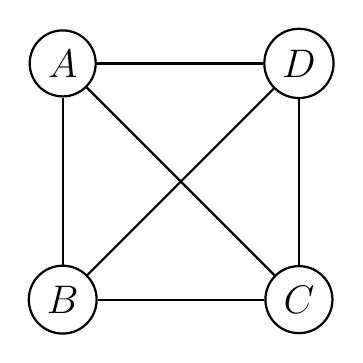
\begin{tikzpicture}[auto, node distance=3cm, every loop/.style={},
                    thick,main node/.style={circle,draw,font=\sffamily\Large\bfseries}]

  \node[main node] (1) {$A$};
  \node[main node] (2) [below of=1] {$B$};
  \node[main node] (3) [right of=2] {$C$};
  \node[main node] (4) [right of=1] {$D$};

  \path[every node/.style={font=\sffamily\small}]
    (1) edge node {} (4)
    	edge node {} (3)
    (2) edge node {} (1)
        edge node {} (4)
    (3) edge node {} (2)
    (4) edge node {} (3);
\end{tikzpicture}
\end{center}

This graph is called a \gls{complete} as every \gls{vertex} is connected to every other \gls{vertex} by an \gls{edge}; in fact this graph in particular is called $K_4$ as it is the complete four vertex graph. We would like to find out if we can draw this above graph without having any lines crossing. We can in fact draw this graph without any intersections and for any skeptics who may being reading this, the below is $k_4$ without any \glspl{edge} intersecting.

\begin{center}
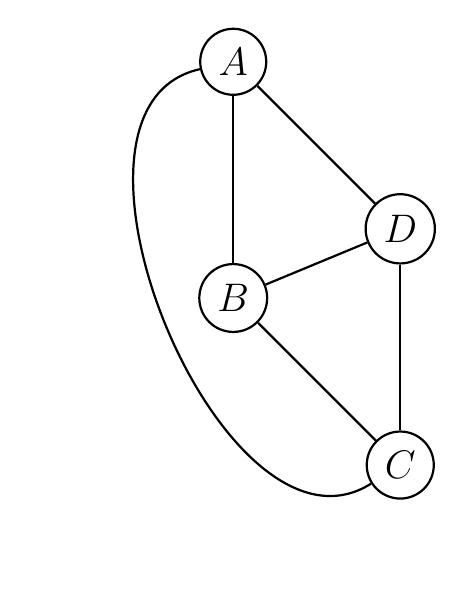
\begin{tikzpicture}[auto, node distance=3cm, every loop/.style={},
                    thick,main node/.style={circle,draw,font=\sffamily\Large\bfseries}]

  \node[main node] (1) {$A$};
  \node[main node] (2) [below of=1] {$B$};
  \node[main node] (3) [below right of=2] {$C$};
  \node[main node] (4) [below right of=1] {$D$};

  \path[every node/.style={font=\sffamily\small}]
    (1) edge node {} (4)
    	edge [bend right = 100]node {} (3)
    (2) edge node {} (1)
        edge node {} (4)
    (3) edge node {} (2)
    (4) edge node {} (3);
\end{tikzpicture}
\end{center}

So if this graph can be drawn without intersection, can any graph be drawn without intersections? If some can and some can't how do we tell which can be drawn and which can not?

\subsection{Kuratowski's Theorem}
Kuratowski's theorem tell us exactly what graphs can be drawn on a plane or sphere. We say either a plane or sphere as it turns out to be the same question. %TODO prove that drawing on plane and sphere is same question
Now before we tackle the theorem let's lay down some terminology.

\subsubsection{Terminology: face}

Consider the following graph.

\begin{center}
	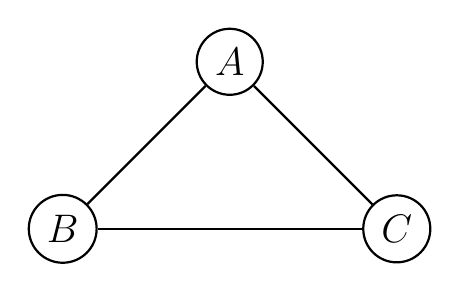
\begin{tikzpicture}[auto, node distance=3cm, every loop/.style={},
	thick,main node/.style={circle,draw,font=\sffamily\Large\bfseries}]
	
	  \node[main node] (1) {$A$};
	  \node[main node] (2) [below left of=1] {$B$};
	  \node[main node] (3) [below right of=1] {$C$};
	  
	  \path[every node/.style={font=\sffamily\small}]
	  (1) edge node {} (2)
		  edge node {} (3)
	  (2) edge node {} (3);
	
	\end{tikzpicture}
\end{center}

We say this graph has two \glspl{face}. One \gls{face} is easy to see and contained within triangle $ABC$. The other \gls{face} is a bit harder to see, however it is all the space outside of the triangle $ABC$. We may call this second face the outer \gls{face} for this drawing of the graph, however it is also possible to draw it such that the inner face may be the outer face. You can think of this as kind of turning the triangle inside out.

A face only makes sense to talk about for a graph that can be embedded in a certain space. For example the graph $K_4$ may look like it has $5$ faces in the following drawing.

\begin{center}
	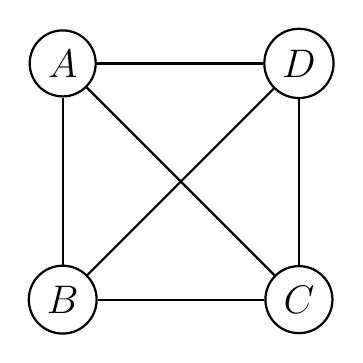
\begin{tikzpicture}[auto, node distance=3cm, every loop/.style={},
	thick,main node/.style={circle,draw,font=\sffamily\Large\bfseries}]
	
	\node[main node] (1) {$A$};
	\node[main node] (2) [below of=1] {$B$};
	\node[main node] (3) [right of=2] {$C$};
	\node[main node] (4) [right of=1] {$D$};
	
	\path[every node/.style={font=\sffamily\small}]
	(1) edge node {} (4)
	edge node {} (3)
	(2) edge node {} (1)
	edge node {} (4)
	(3) edge node {} (2)
	(4) edge node {} (3);
	\end{tikzpicture}
\end{center}
This would be wrong as a face assumes a drawing without \glspl{edge} intersecting. This can be rectified if the graph can be drawn without intersection and thus we find this drawing.
\begin{center}
	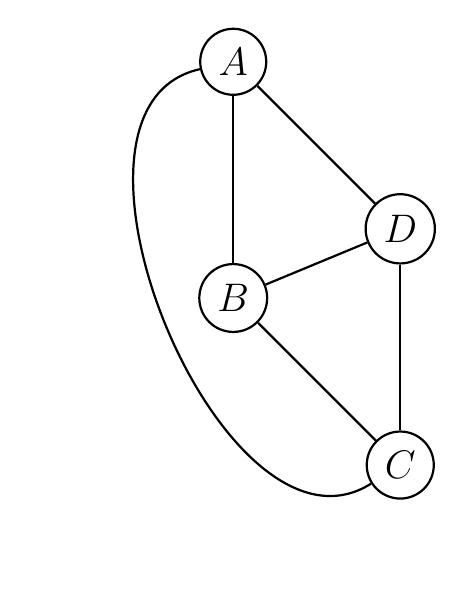
\begin{tikzpicture}[auto, node distance=3cm, every loop/.style={},
	thick,main node/.style={circle,draw,font=\sffamily\Large\bfseries}]
	
	\node[main node] (1) {$A$};
	\node[main node] (2) [below of=1] {$B$};
	\node[main node] (3) [below right of=2] {$C$};
	\node[main node] (4) [below right of=1] {$D$};
	
	\path[every node/.style={font=\sffamily\small}]
	(1) edge node {} (4)
	edge [bend right = 100]node {} (3)
	(2) edge node {} (1)
	edge node {} (4)
	(3) edge node {} (2)
	(4) edge node {} (3);
	\end{tikzpicture}
\end{center}
This means there are actually $4$ \glspl{face} in $k_4$.

\subsubsection{Terminology: contraction}

Let us consider the following graph.

\begin{center}
	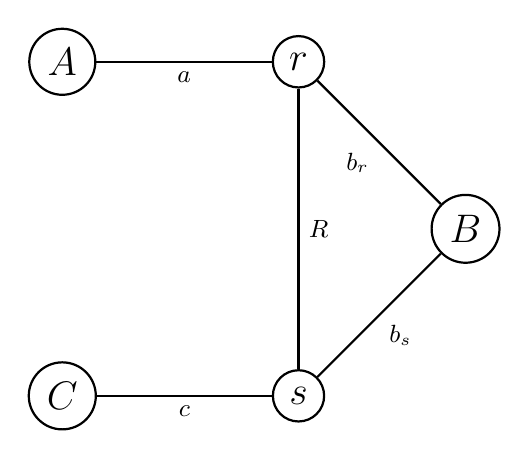
\begin{tikzpicture}[auto, node distance=3cm, every loop/.style={},
	thick,main node/.style={circle,draw,font=\sffamily\Large\bfseries}]
	
	\node[main node] (1) {$r$};
	\node[main node] (2) [below right of=1] {$B$};
	\node[main node] (3) [left of=1] {$A$};
	\node[main node] (4) [below left of=2] {$s$};
	\node[main node] (5) [left of=4] {$C$};
	
	\path[every node/.style={font=\sffamily\small}]
	(1) edge node {$R$} (4)
	edge node {$a$} (3)
	(2) edge node {$b_r$} (1)
	edge node {$b_s$} (4)
	(4) edge node {$c$} (5);
	\end{tikzpicture}
\end{center}

We wish to preform a \gls{contraction} on \gls{edge} $R$. To be clear all graph \glspl{contraction} are on \glspl{edge}. So we will make a new \gls{vertex}, $r\cdot s$ which has all the \glspl{edge} of $r$ and all the \glspl{edge} of $s$ except the \gls{edge} we are contracting across. In this case the \gls{edge} we are contracting across is $R$ and thus we get the following \gls{multigraph}.

\begin{center}
	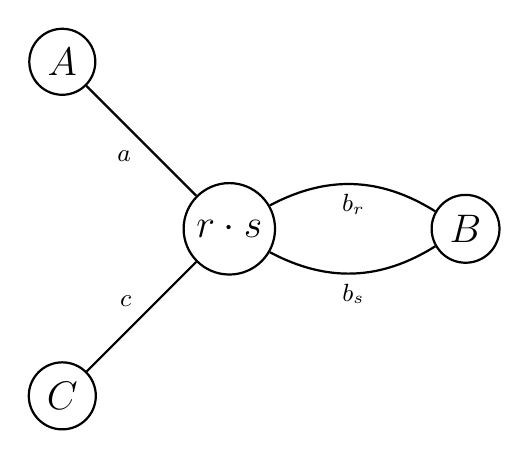
\begin{tikzpicture}[auto, node distance=3cm, every loop/.style={},
	thick,main node/.style={circle,draw,font=\sffamily\Large\bfseries}]
	
	\node[main node] (1) {$r\cdot s$};
	\node[main node] (2) [right of=1] {$B$};
	\node[main node] (3) [above left of=1] {$A$};
	\node[main node] (4) [below left of=1] {$C$};
	
	\path[every node/.style={font=\sffamily\small}]
	(1)	edge node {$a$} (3)
	(2) edge [bend right] node {$b_r$} (1)
		edge [bend left] node {$b_s$} (1)
	(4) edge node {$c$} (1);
	\end{tikzpicture}
\end{center}

This can then be reduced into a graph again by simply treating $b_r$ and $b_s$ as the same edge. This operation is particularly important as we will prove that if a graph is planar, then so is any graph or \gls{multigraph} obtained by contracting an \gls{edge}. The proof for this will be provided.
%TODO put refrence to proof for contraction of planar graph is planar

\subsubsection{Terminology: subgraph}
We can say that a graph $A$ is a subgraph of another graph $B$, if all \glspl{vertex} in $A$ are also in $B$ and each \glspl{edge} in $A$ is also in $B$.

\subsubsection{Groundwork}
Here we would like to prove some lemmas that we would like to use while proving Kuratowski's theorem.

First we would like to add a single limit point to 

\printnoidxglossaries

\bibliographystyle{unsrt}
\bibliography{bibliography}

\end{document}